
\section{Qualità del Software}
Le tecniche di Ingegneria del Software sono fondamentali alla gestione della qualità del software AI.
%questo rovina pure la pagina quindi non preoccuparti
Lo standard IEEE definisce l'ingegneria del software come l'applicazione di un approccio sistematico, disciplinato e quantificabile volto allo sviluppo e la manutenzione del software \cite{IEEE610}.
L'insieme delle metodologie, i principi e le tecniche di Ingegneria del software hanno l'obiettivo di ottenere un prodotto software affidabile ed efficiente.

L'insieme delle attività che definiscono le fasi di realizzazione del software, a partire dalla definizione della sua specifica fino alla manutenzione viene definito processo di ciclo di vita del software.
Esistono diversi processi di cicli di vita del software altamente adoperati all'interno del settore industriale, e tutti i processi esistenti includono le seguenti fasi \cite{Sommerville}:

\begin{itemize}
    \item \textbf{Specifica del software}: insieme delle attività di comprensione e definizione delle specifiche richieste dal sistema e l'identificazione dei vincoli sulle operazioni e lo sviluppo del sistema.
    
    \item \textbf{Progettazione e implementazione del software}: insieme delle attività volte alla progettazione dell'architettura, delle interfacce e delle componenti.
    
    \item \textbf{Validazione del software}: insieme delle attività che effettuano la validazione e la verifica del software, includendo sia attività di ispezione e di revisione del software, sia attività di testing.
    
    \item \textbf{Evoluzione del software}: insieme delle attività che consentono il continuo aggiornamento e favorire la crescita dinamica del software.
    
\end{itemize}
Ognuna di queste fasi prevede una serie di attività utili al supporto della realizzazione del progetto. In particolare, è necessario notare che ogni fase viene supportata da attività di pianificazione del progetto, di monitoraggio e di tracciabilità degli artefatti.
Una delle più importanti attività che viene svolta durante la fase di monitoraggio del sistema software è la valutazione della qualità.

Una definizione importante e precisa da considerare quando si interagisce con la qualità del software è quella definita dallo Standard ISO/IEC 25010:2011 \cite{ieee25010}.
Essa viene definita come \textit{"la capacità del software di soddisfare le esigenze dichiarate e implicite sotto specifiche condizioni quando utilizzato"}.
Queste particolari esigenze da soddisfare sono state definite dai modelli di qualità, i quali hanno lo scopo di effettuare una categorizzazione della qualità del software tramite un'insieme di caratteristiche.
Successivamente queste caratteristiche sono ulteriormente scomposte ciclicamente in sottocaratteristiche e proprietà.
Ogni definizione di sottoinsieme di caratteristiche ha lo scopo di poter ottenere una rappresentazione dettagliata di un aspetto della qualità del software, a tal punto da renderlo misurabile. In figura \ref{fig:quality_model_def} è possibile osservare come dalla definizione generica di un aspetto della qualità del software è possibile quindi andare a definire delle proprietà che sono direttamente misurabili.
\begin{figure}[h]
    \centering
    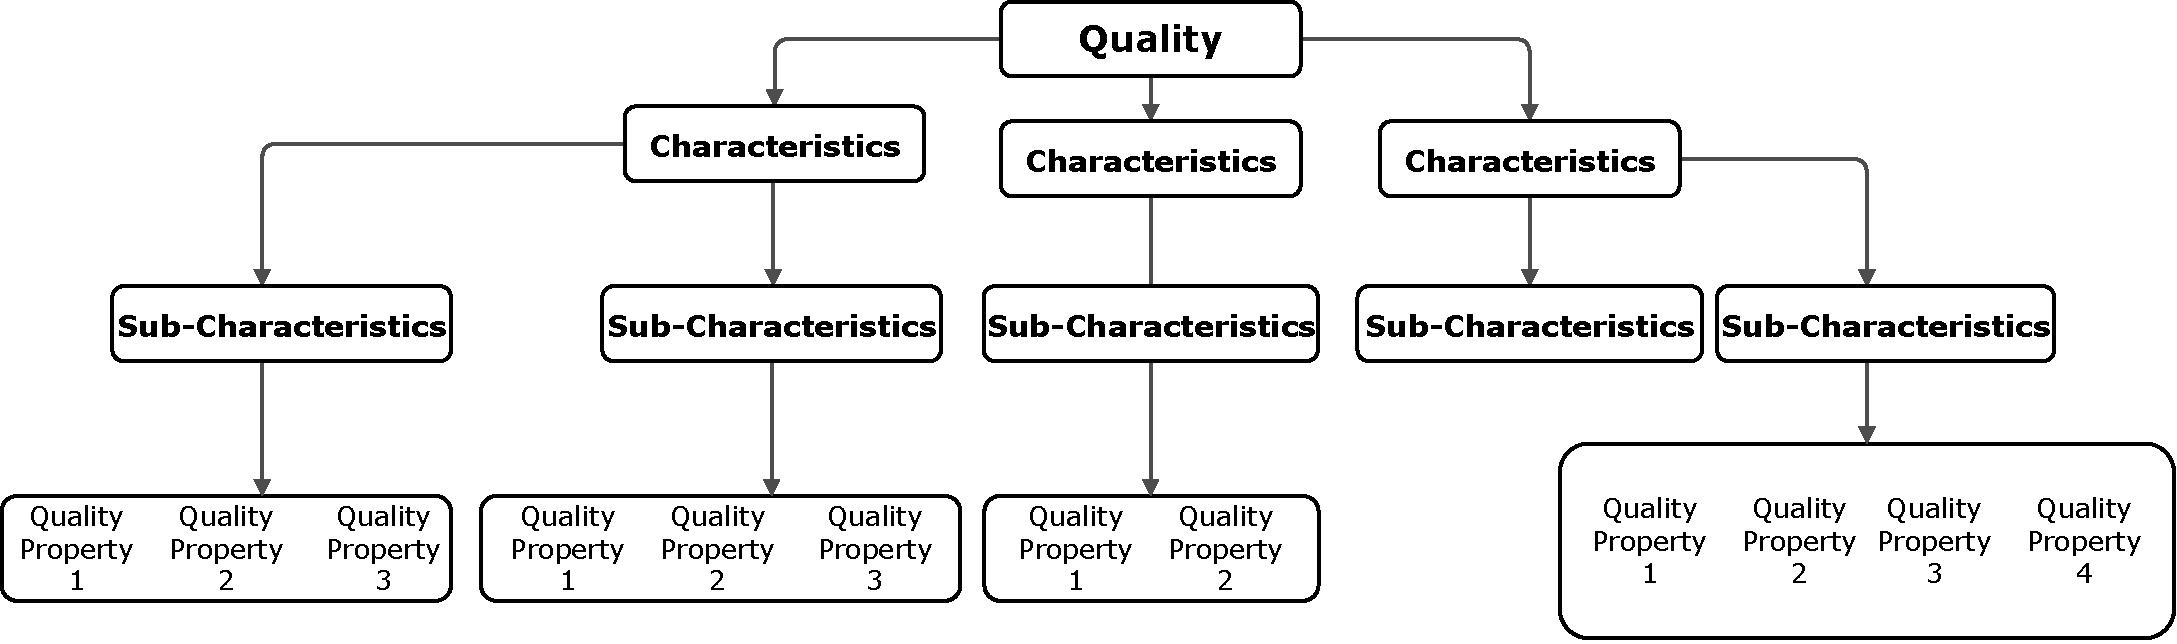
\includegraphics[width=1\textwidth]{Figure/Background/quality_def.pdf}
    \caption{Struttura utilizzata per la definizione di modelli di qualità}
    \label{fig:quality_model_def}
\end{figure}

Tra i modelli maggiormente utilizzati per la gestione della qualità del software è presente il modello ISO/IEC 9126.
%continuare con la definizione tramite ref mendeley isoiec 9126

\subsection{ISO/IEC 9126}
Le norme proposte all'interno del modello \textit{ISO/IEC 9126} sono emesse dall'ISO, l'organismo internazionale di standardizzazione (International Organization for Standardization) e, in particolare, dall'organo interno del settore delle tecnologie e della comunicazione (IEC, International Electrotechnical Commission).
Le norme emesse quindi definiscono la qualità del software in quattro parti: 
\begin{enumerate}
    \item Modello di qualità del software.
    \item Metriche per la qualità esterna.
    \item Metriche per la qualità interna.
    \item Metriche per la qualità in uso.
\end{enumerate}

La qualità del software è particolarmente legata alla maturità del processo definito al fine dello sviluppo.
E' importante quindi definire una relazione tra le diverse tipologie di qualità presenti nel modello di qualità.
Dall'insieme di relazioni che collegano la qualità del processo alla qualità del prodotto, come raffigurato in figura \ref{fig:quality_cycle_9126}, è possibile evincere che migliorare aspetti di qualità del processo possono influenzare positivamente aspetti della qualità del prodotto. A sua volta il miglioramento della qualità interna, e quindi indirettamente includendo la qualità esterna del prodotto, porta benefici alla qualità in uso del prodotto.
Inoltre, seguendo direttamente le relazioni in senso inverso, è possibile valutare la qualità in uso al fine di avere un sistema di feedback che fornisce informazioni sull'effetto dei miglioramenti apportati, a sua volta utili per il miglioramento del processo.



Gli attributi interni del software, quindi, sono un prerequisito fondamentale per analizzare anche altri aspetti della qualità del software, come le caratteristiche esterne del prodotto, rappresentano un prerequisito fondamentale per analizzare la qualità in uso desiderata.

Il modello di qualità del software quindi è definito da un insieme di caratteristiche che riguardano diversi aspetti del software, dove in ciascuna caratteristica sono a sua volta definite sottocaratteristiche. 
In particolare, analizzando il modello \textit{ISO/IEC 9126}, la qualità è modellata dalla definizione di 6 caratteristiche, strutturate come in Tabella \ref{tab:iso_iec9126}.

\begin{figure}[h]
    \centering
    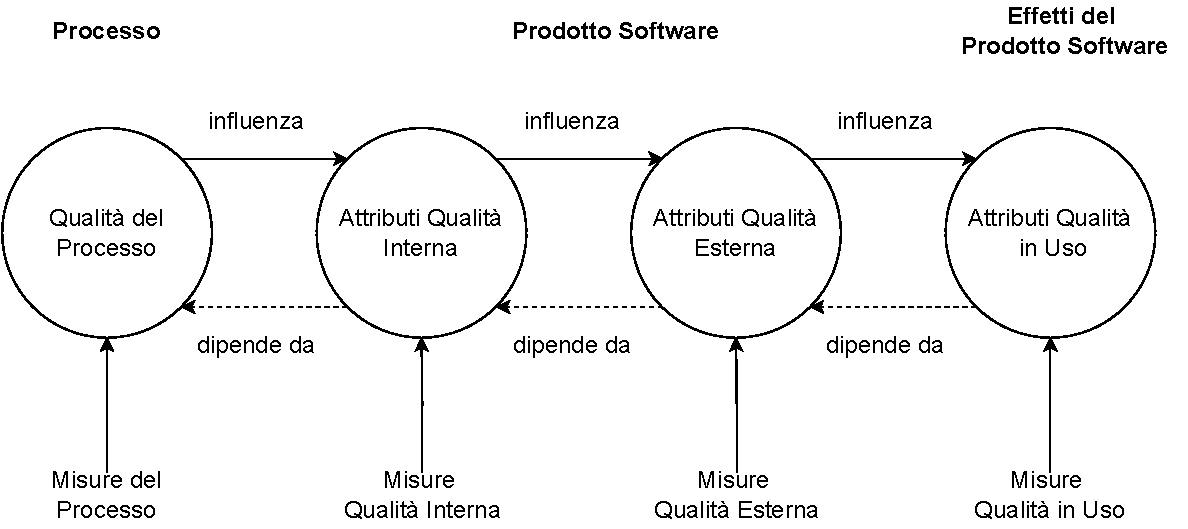
\includegraphics[width=\textwidth]{Figure/Background/quality_cycle_process.pdf}
    \caption{Ciclo di sviluppo della qualità del prodotto software}
    \label{fig:quality_cycle_9126}
\end{figure}

\begin{table}[h!]
\centering
    \begin{tabular}{|c|p{6cm}|}
        \hline
        \textbf{Caratteristiche} & \textbf{Attributi}\\
        \hline
        Funzionalità (Functionality) & Completezza, Accuratezza, Interoperabilità, Sicurezza, Aderenza alla funzionalità. \\
        \hline
        Affidabilità (Reliability) & Maturità, Tolleranza ai guasti, Recuperabilità, Aderenza all'affidabilità.\\
        \hline
        Usabilità (Usability) & Comprensibilità, Apprendibilità, Operabilità, Attrattività, Aderenza all'usabilità. \\
        \hline
        Efficienza (Efficiency) & Comportamento sul tempo di esecuzione, Utilizzo delle risorse, Aderenza all'efficienza. \\
        \hline
        Manutenibilità (Maintainability) & Analizzabilità, Modificabilità, Stabilità, Provabilità, Aderenza alla manutenibilità.\\
        \hline
        Portabilità (Portability) & Adattabilità, Installabilità, Coesistenza, Sostituibilità, Aderenza alla portabilità.\\
        \hline
        Qualità in uso (Quality in use) & Efficacia, Produttività, Sicurezza, Soddisfazione.\\
        \hline
    \end{tabular}
    \caption{Modello di qualità ISO/IEC 9126}
    \label{tab:iso_iec9126}
\end{table}